\documentclass{article}
\usepackage{graphicx}
\usepackage{float}
\title{COMP7906A Introduction to Cyber Security Assignment 1}
\author{Wang Dingrui}
\date{\today}

\begin{document}

\maketitle

\section{Question 1 (codes in the appendix)}
% Your answer to question 1 goes here


\begin{figure}[H]
    \makebox[\textwidth][c]{
        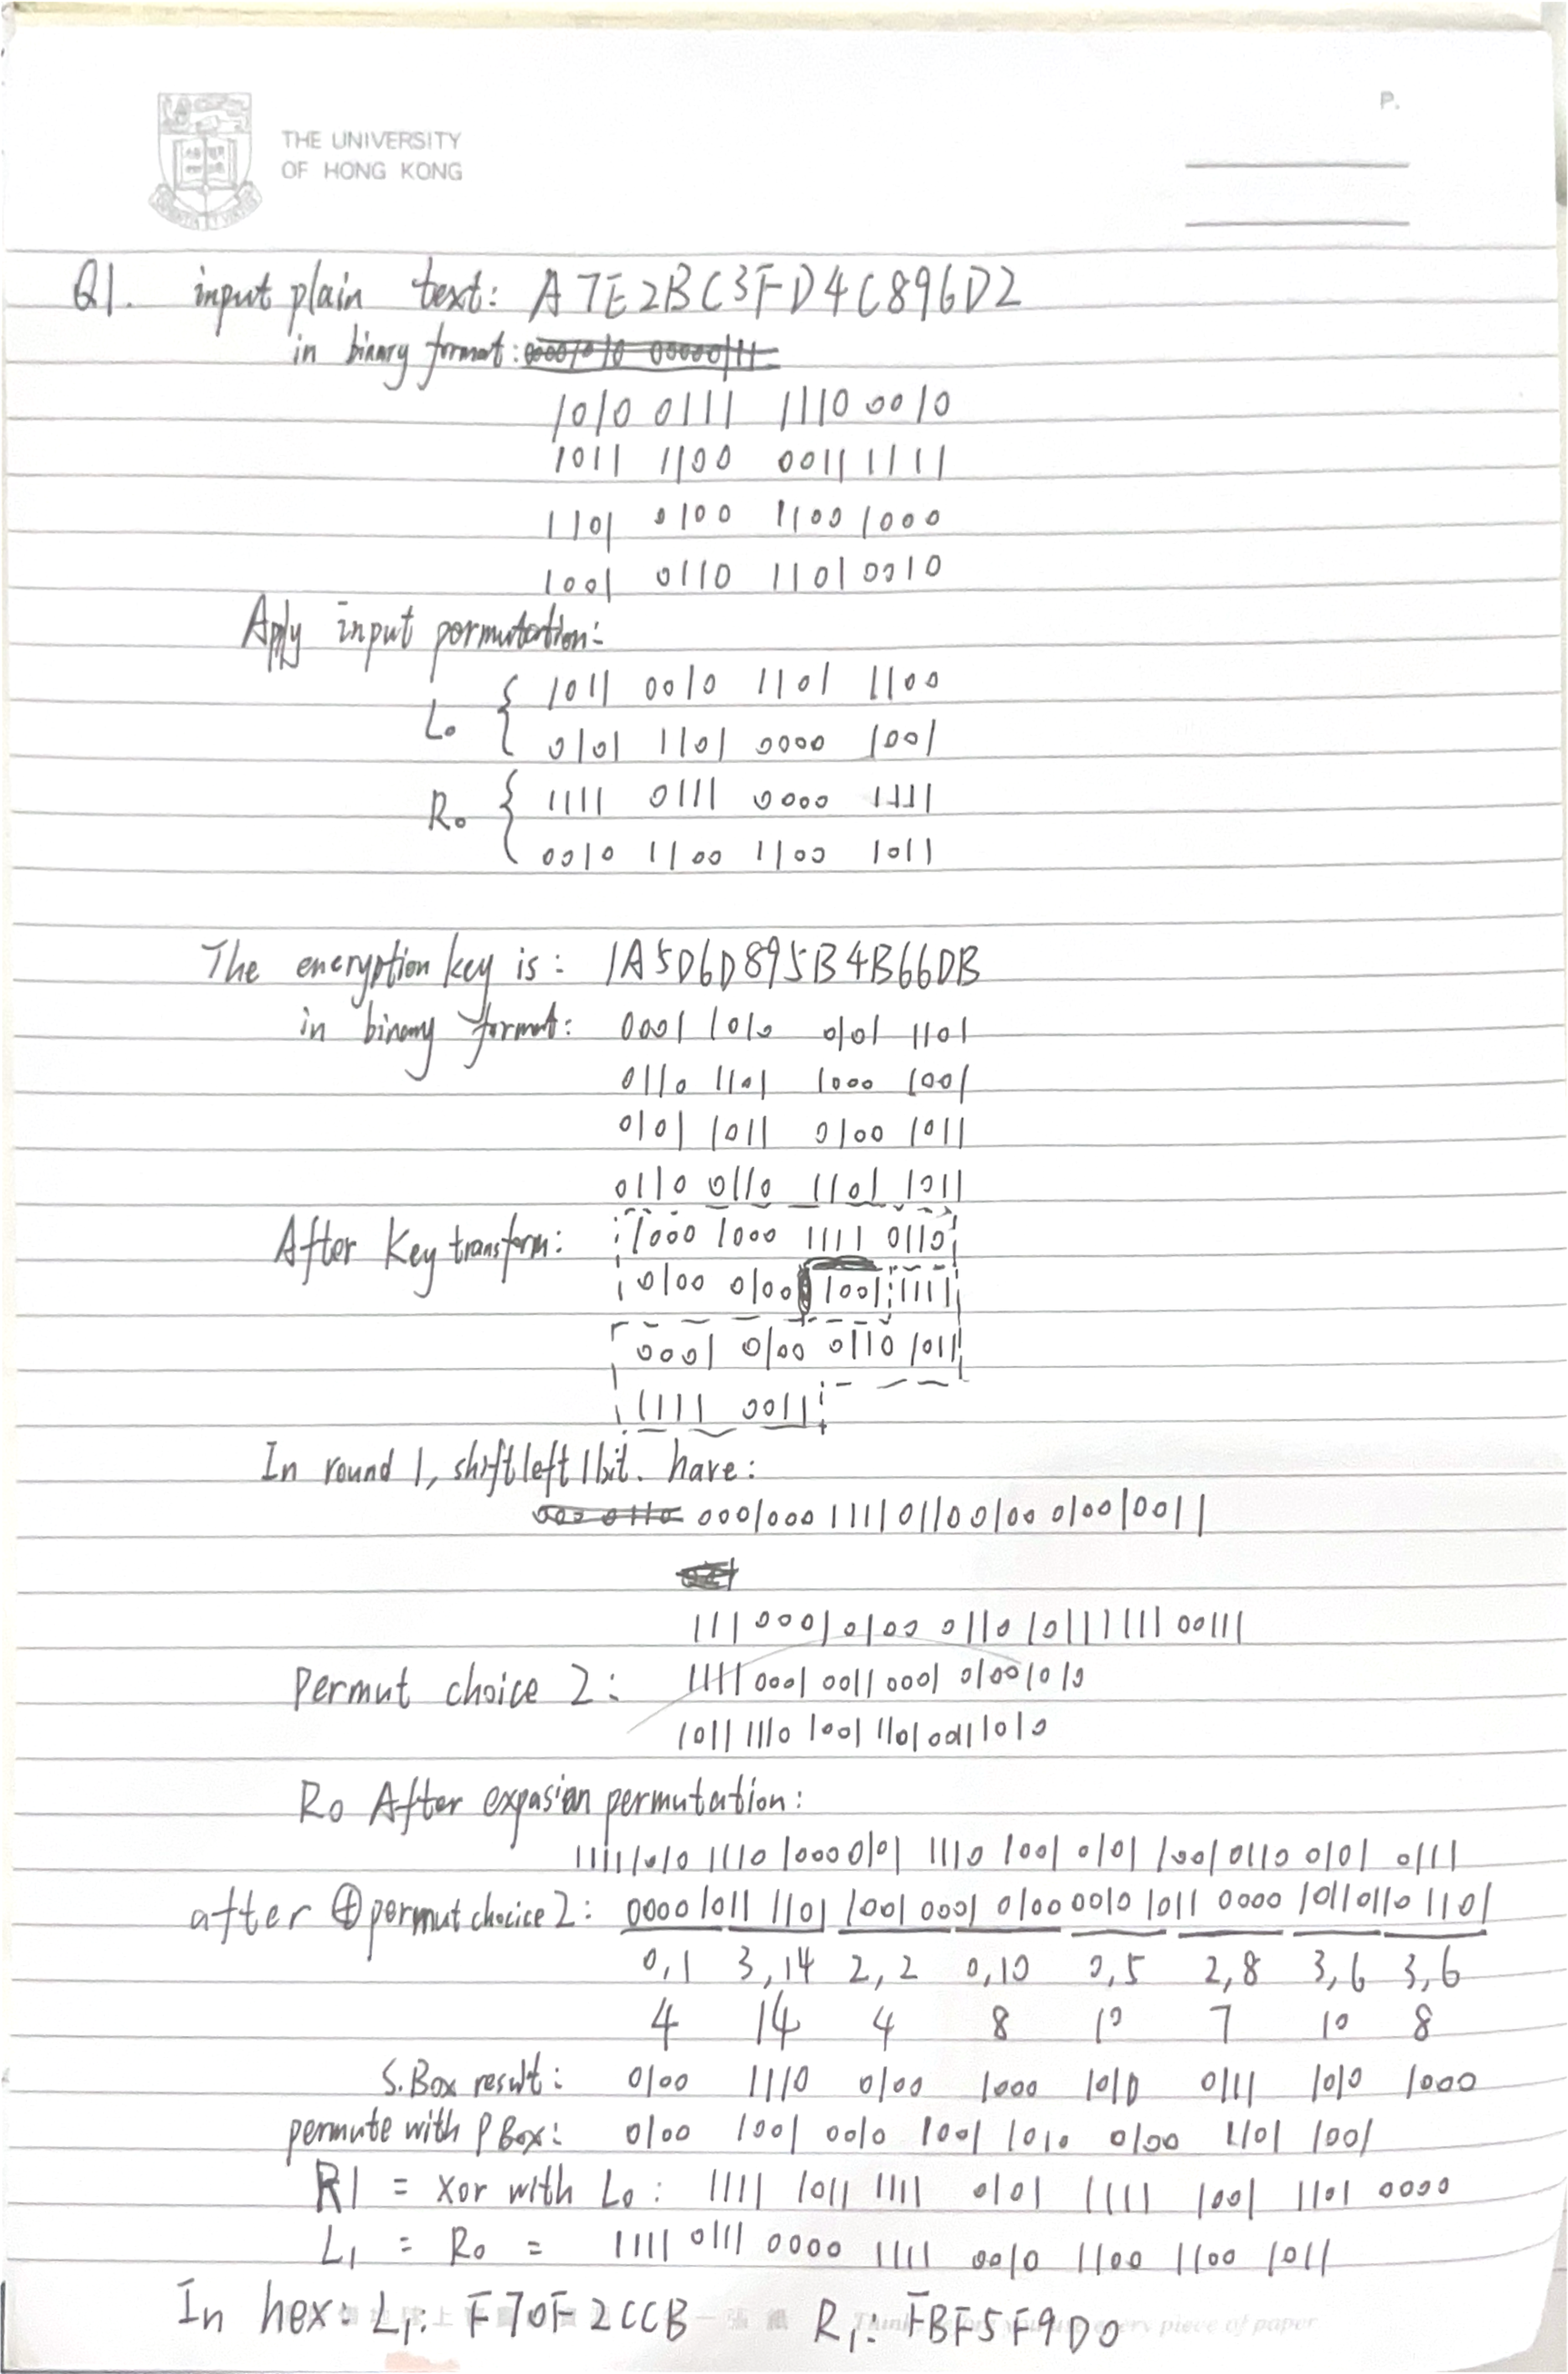
\includegraphics[width=1.2\textwidth]{q1handwriting.pdf}
    }
    \caption{Answer to Question 1}
    \label{fig:q1handwriting}
\end{figure}





\section{Question 2}
% Your answer to question 2 goes here

\section{Question 3}
% Your answer to question 3 goes here

% Add more sections for additional questions if needed

\section{Appendix}

\subsection{Q1 codes}
\begin{verbatim}

def getBinMat(s):
    mat = ""
    for i in range(len(s)):
        mat += bin(eval("0x"+s[i]))[2:].zfill(4)
    for i in range(len(mat)):
        if i % 4 == 0:
            print(" ", end="")
        if i % 16 == 0:
            print()
        print(mat[i],end="")
    return mat

def permute(mat, p):
    mat2 = ""
    for i in range(len(p)):
        mat2 += mat[p[i]-1]
    return mat2

def shift_left(mat, n):
    return mat[n:] + mat[:n]

def xor(mat1, mat2):
    return "".join([str(int(mat1[i]) ^ int(mat2[i])) for i in range(len(mat1))])

input_permutation = [58, 50, 42, 34, 26, 18, 10, 2,
                        60, 52, 44, 36, 28, 20, 12, 4,
                        62, 54, 46, 38, 30, 22, 14, 6,
                        64, 56, 48, 40, 32, 24, 16, 8,
                        57, 49, 41, 33, 25, 17, 9, 1,
                        59, 51, 43, 35, 27, 19, 11, 3,
                        61, 53, 45, 37, 29, 21, 13, 5,
                        63, 55, 47, 39, 31, 23, 15, 7]

key_permutation = [57, 49, 41, 33, 25, 17, 9,
                    1, 58, 50, 42, 34, 26, 18,
                    10, 2, 59, 51, 43, 35, 27,
                    19, 11, 3, 60, 52, 44, 36,
                    63, 55, 47, 39, 31, 23, 15,
                    7, 62, 54, 46, 38, 30, 22,
                    14, 6, 61, 53, 45, 37, 29,
                    21, 13, 5, 28, 20, 12, 4]

key_permutation_2 = [14, 17, 11, 24, 1, 5,
                        3, 28, 15, 6, 21, 10,
                        23, 19, 12, 4, 26, 8,
                        16, 7, 27, 20, 13, 2,
                        41, 52, 31, 37, 47, 55,
                        30, 40, 51, 45, 33, 48,
                        44, 49, 39, 56, 34, 53,
                        46, 42, 50, 36, 29, 32]

expansion_permutation = [32, 1, 2, 3, 4, 5,
                         4, 5, 6, 7, 8, 9,
                         8, 9, 10, 11, 12, 13,
                         12, 13, 14, 15, 16, 17,
                            16, 17, 18, 19, 20, 21,
                            20, 21, 22, 23, 24, 25,
                            24, 25, 26, 27, 28, 29,
                            28, 29, 30, 31, 32, 1]

s_box_1 = [[14, 4, 13, 1, 2, 15, 11, 8, 3, 10, 6, 12, 5, 9, 0, 7],
            [0, 15, 7, 4, 14, 2, 13, 1, 10, 6, 12, 11, 9, 5, 3, 8],
            [4, 1, 14, 8, 13, 6, 2, 11, 15, 12, 9, 7, 3, 10, 5, 0],
            [15, 12, 8, 2, 4, 9, 1, 7, 5, 11, 3, 14, 10, 0, 6, 13]]

s_box_2 = [[15, 1, 8, 14, 6, 11, 3, 4, 9, 7, 2, 13, 12, 0, 5, 10],
            [3, 13, 4, 7, 15, 2, 8, 14, 12, 0, 1, 10, 6, 9, 11, 5],
            [0, 14, 7, 11, 10, 4, 13, 1, 5, 8, 12, 6, 9, 3, 2, 15],
            [13, 8, 10, 1, 3, 15, 4, 2, 11, 6, 7, 12, 0, 5, 14, 9]]

s_box_3 = [[10, 0, 9, 14, 6, 3, 15, 5, 1, 13, 12, 7, 11, 4, 2, 8],
            [13, 7, 0, 9, 3, 4, 6, 10, 2, 8, 5, 14, 12, 11, 15, 1],
            [13, 6, 4, 9, 8, 15, 3, 0, 11, 1, 2, 12, 5, 10, 14, 7],
            [1, 10, 13, 0, 6, 9, 8, 7, 4, 15, 14, 3, 11, 5, 2, 12]]

s_box_4 = [[7, 13, 14, 3, 0, 6, 9, 10, 1, 2, 8, 5, 11, 12, 4, 15],
            [13, 8, 11, 5, 6, 15, 0, 3, 4, 7, 2, 12, 1, 10, 14, 9],
            [10, 6, 9, 0, 12, 11, 7, 13, 15, 1, 3, 14, 5, 2, 8, 4],
            [3, 15, 0, 6, 10, 1, 13, 8, 9, 4, 5, 11, 12, 7, 2, 14]]

s_box_5 = [[2, 12, 4, 1, 7, 10, 11, 6, 8, 5, 3, 15, 13, 0, 14, 9],
            [14, 11, 2, 12, 4, 7, 13, 1, 5, 0, 15, 10, 3, 9, 8, 6],
            [4, 2, 1, 11, 10, 13, 7, 8, 15, 9, 12, 5, 6, 3, 0, 14],
            [11, 8, 12, 7, 1, 14, 2, 13, 6, 15, 0, 9, 10, 4, 5, 3]]

s_box_6 = [[12, 1, 10, 15, 9, 2, 6, 8, 0, 13, 3, 4, 14, 7, 5, 11],
            [10, 15, 4, 2, 7, 12, 9, 5, 6, 1, 13, 14, 0, 11, 3, 8],
            [9, 14, 15, 5, 2, 8, 12, 3, 7, 0, 4, 10, 1, 13, 11, 6],
            [4, 3, 2, 12, 9, 5, 15, 10, 11, 14, 1, 7, 6, 0, 8, 13]]

s_box_7 = [[4, 11, 2, 14, 15, 0, 8, 13, 3, 12, 9, 7, 5, 10, 6, 1],
            [13, 0, 11, 7, 4, 9, 1, 10, 14, 3, 5, 12, 2, 15, 8, 6],
            [1, 4, 11, 13, 12, 3, 7, 14, 10, 15, 6, 8, 0, 5, 9, 2],
            [6, 11, 13, 8, 1, 4, 10, 7, 9, 5, 0, 15, 14, 2, 3, 12]]
s_box_8 = [[13, 2, 8, 4, 6, 15, 11, 1, 10, 9, 3, 14, 5, 0, 12, 7],
            [1, 15, 13, 8, 10, 3, 7, 4, 12, 5, 6, 11, 0, 14, 9, 2],
            [7, 11, 4, 1, 9, 12, 14, 2, 0, 6, 10, 13, 15, 3, 5, 8],
            [2, 1, 14, 7, 4, 10, 8, 13, 15, 12, 9, 0, 3, 5, 6, 11]]

s_boxes = [s_box_1, s_box_2, s_box_3, s_box_4, s_box_5, s_box_6, s_box_7, s_box_8]

p_box_permutation = [16, 7, 20, 21, 29, 12, 28, 17,
                     1, 15, 23, 26, 5, 18, 31, 10,
                        2, 8, 24, 14, 32, 27, 3, 9,
                        19, 13, 30, 6, 22, 11, 4, 25]

if __name__ == "__main__":
    s = "A7E2BC3FD4C896D2"
    s_mat = getBinMat(s)
    
    s_init_perm = permute(s_mat, input_permutation)
    l0 = s_init_perm[:32]
    r0 = s_init_perm[32:]
    print("\n\n")
    for i in range(len(s_init_perm)):
        if i % 4 == 0:
            print(" ", end="")
        if i % 16 == 0:
            print()
        print(s_init_perm[i],end="")
        
    key = "1A5D6D895B4B66DB"
    print("\n\n")
    print("key: ", key)
    
    key_mat = getBinMat(key)
    key_perm = permute(key_mat, key_permutation)
    print("\n\n")
    for i in range(len(key_perm)):
        if i % 4 == 0:
            print(" ", end="")
        if i % 16 == 0:
            print()
        print(key_perm[i],end="")
        
    key_left = key_perm[:28]
    key_right = key_perm[28:]
    print("\n\n")
    
    key_left_shift = shift_left(key_left, 1)
    key_right_shift = shift_left(key_right, 1)
    
    print("key_left_shift: ", key_left_shift)
    print("key_right_shift: ", key_right_shift)
    
    key_shifted = key_left_shift + key_right_shift
    
    key_perm_2 = permute(key_shifted, key_permutation_2)
    print("key_perm_2: ")
    
    print(key_perm_2[:24])
    print(key_perm_2[24:])
    
    expanded_r0 = permute(r0, expansion_permutation)
    
    print("expanded_r0: ", expanded_r0)
    
    
    xor_result = xor(expanded_r0, key_perm_2)
    print("expanded_r0 ^ key_perm_2: ", xor_result)
    
    s_box_result = ""
    for i in range(8):
        sb_input = xor_result[i*6:(i+1)*6]
        row_num = int(sb_input[0] + sb_input[5], 2)
        col_num = int(sb_input[1:5], 2)
        target = s_boxes[i][row_num][col_num]
        bin_target = bin(target)[2:].zfill(4)   
        s_box_result += bin_target
        print("sb_input: ", sb_input, "row_num: ", row_num, "col_num: ", col_num, "target: ", target, bin_target)

    print("s_box_result: ", s_box_result)
    
    p_box_result = permute(s_box_result, p_box_permutation)
    print("p_box_result: ", p_box_result)
    
    xor_result_2 = xor(p_box_result, l0)
    
    print("r1 = xor with l0: ", xor_result_2, "In hex per 4 bit: ", hex(int(xor_result_2, 2)).upper()[2:])

    print("l1 = r0: ", r0, "In hex per 4 bit: ", hex(int(r0, 2)).upper()[2:])
    
        
        
        
\end{verbatim}

\end{document}